\section{Pfsense}

Démarrer la machine virtuelle Pfsense, comme sur la figure suivante :
\begin{figure}[h!]
	\begin{center}
		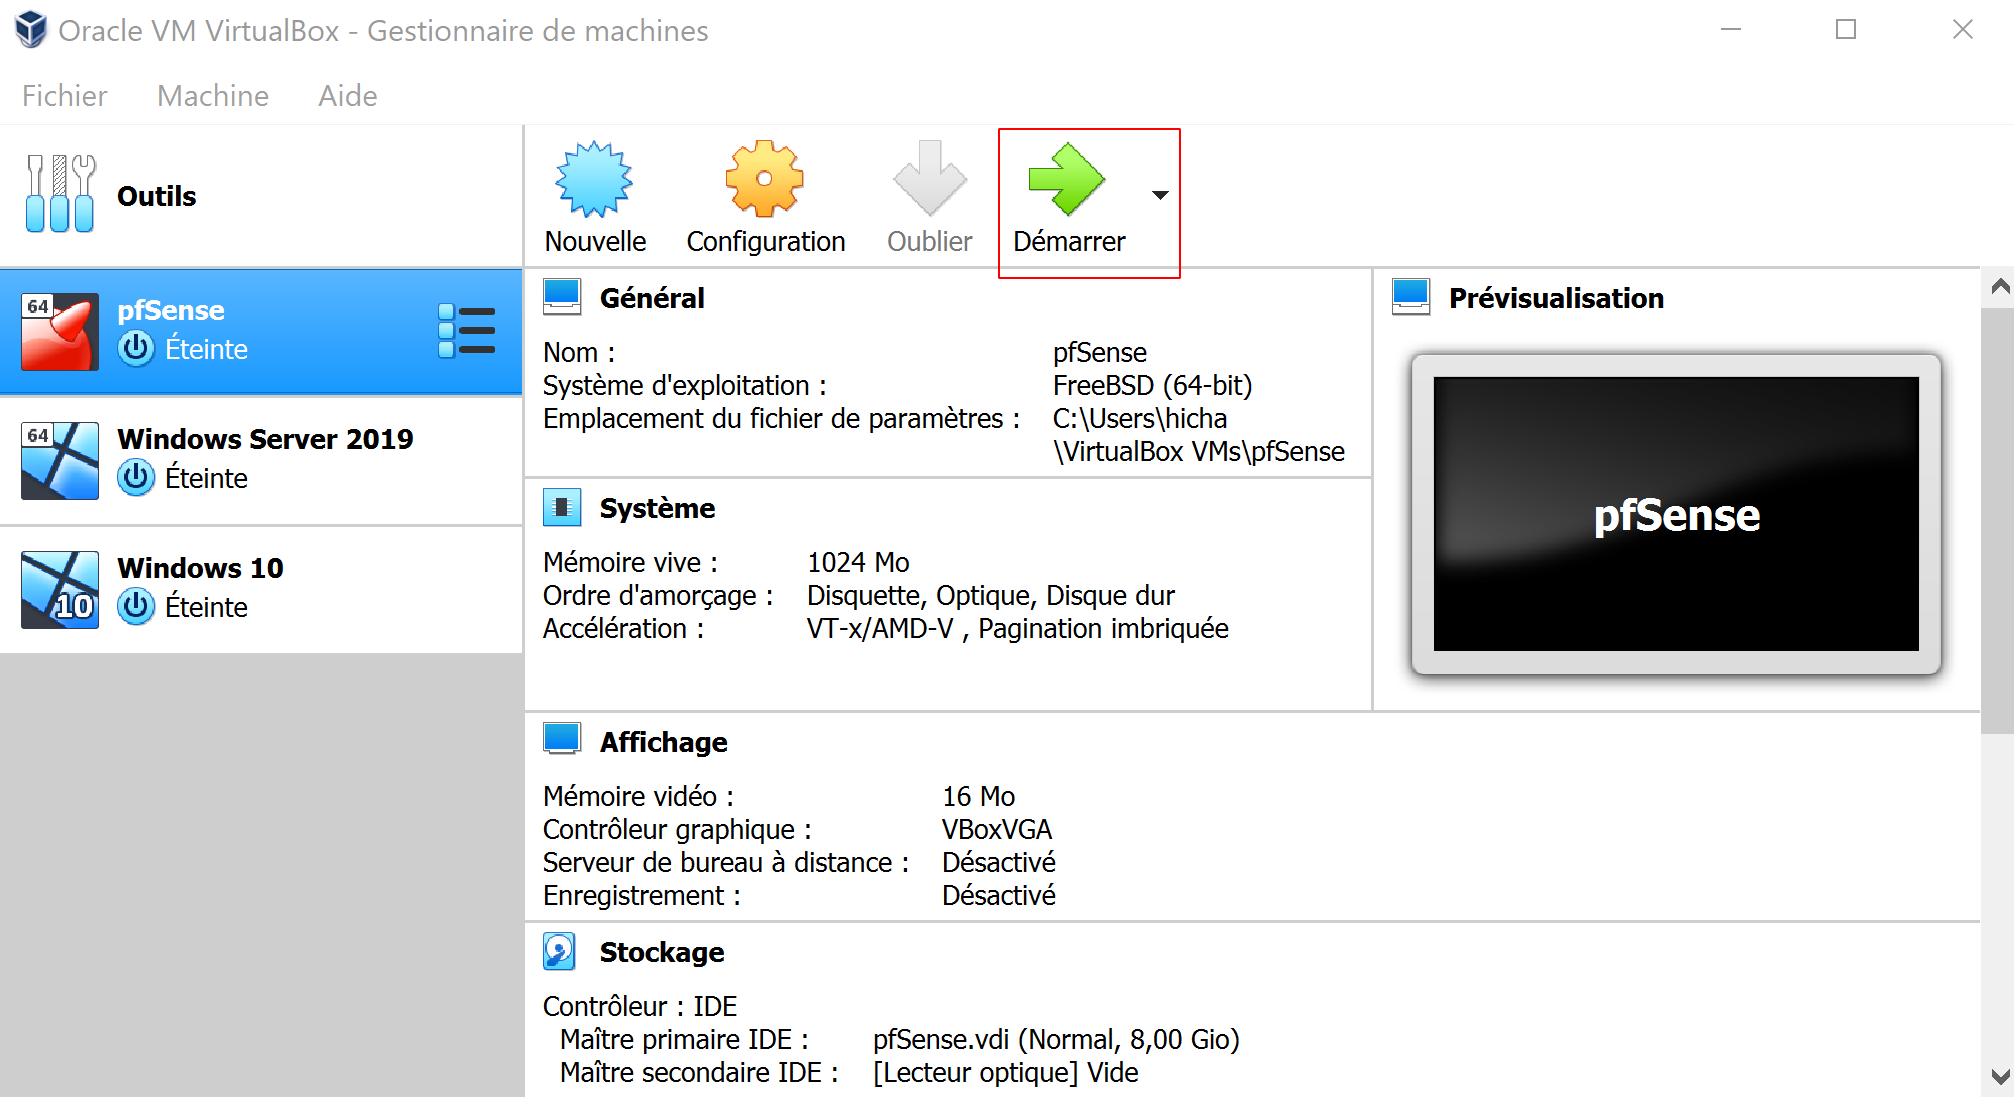
\includegraphics[scale=0.7]{Pfsense_Screeshots/14.png}
		\caption{Démarrage de la machine virtuelle Pfsense}
		\label{Pfsense_Screeshots/14}
	\end{center}
\end{figure}
\FloatBarrier 

\newpage
\subsection{Configuration des adresses IP}

Sélectionner l'option de configuration des interfaces IP, en tapant \textbf{2}, puis appuyer sur la touche \textbf{Entrée} :
\begin{figure}[h!]
	\begin{center}
		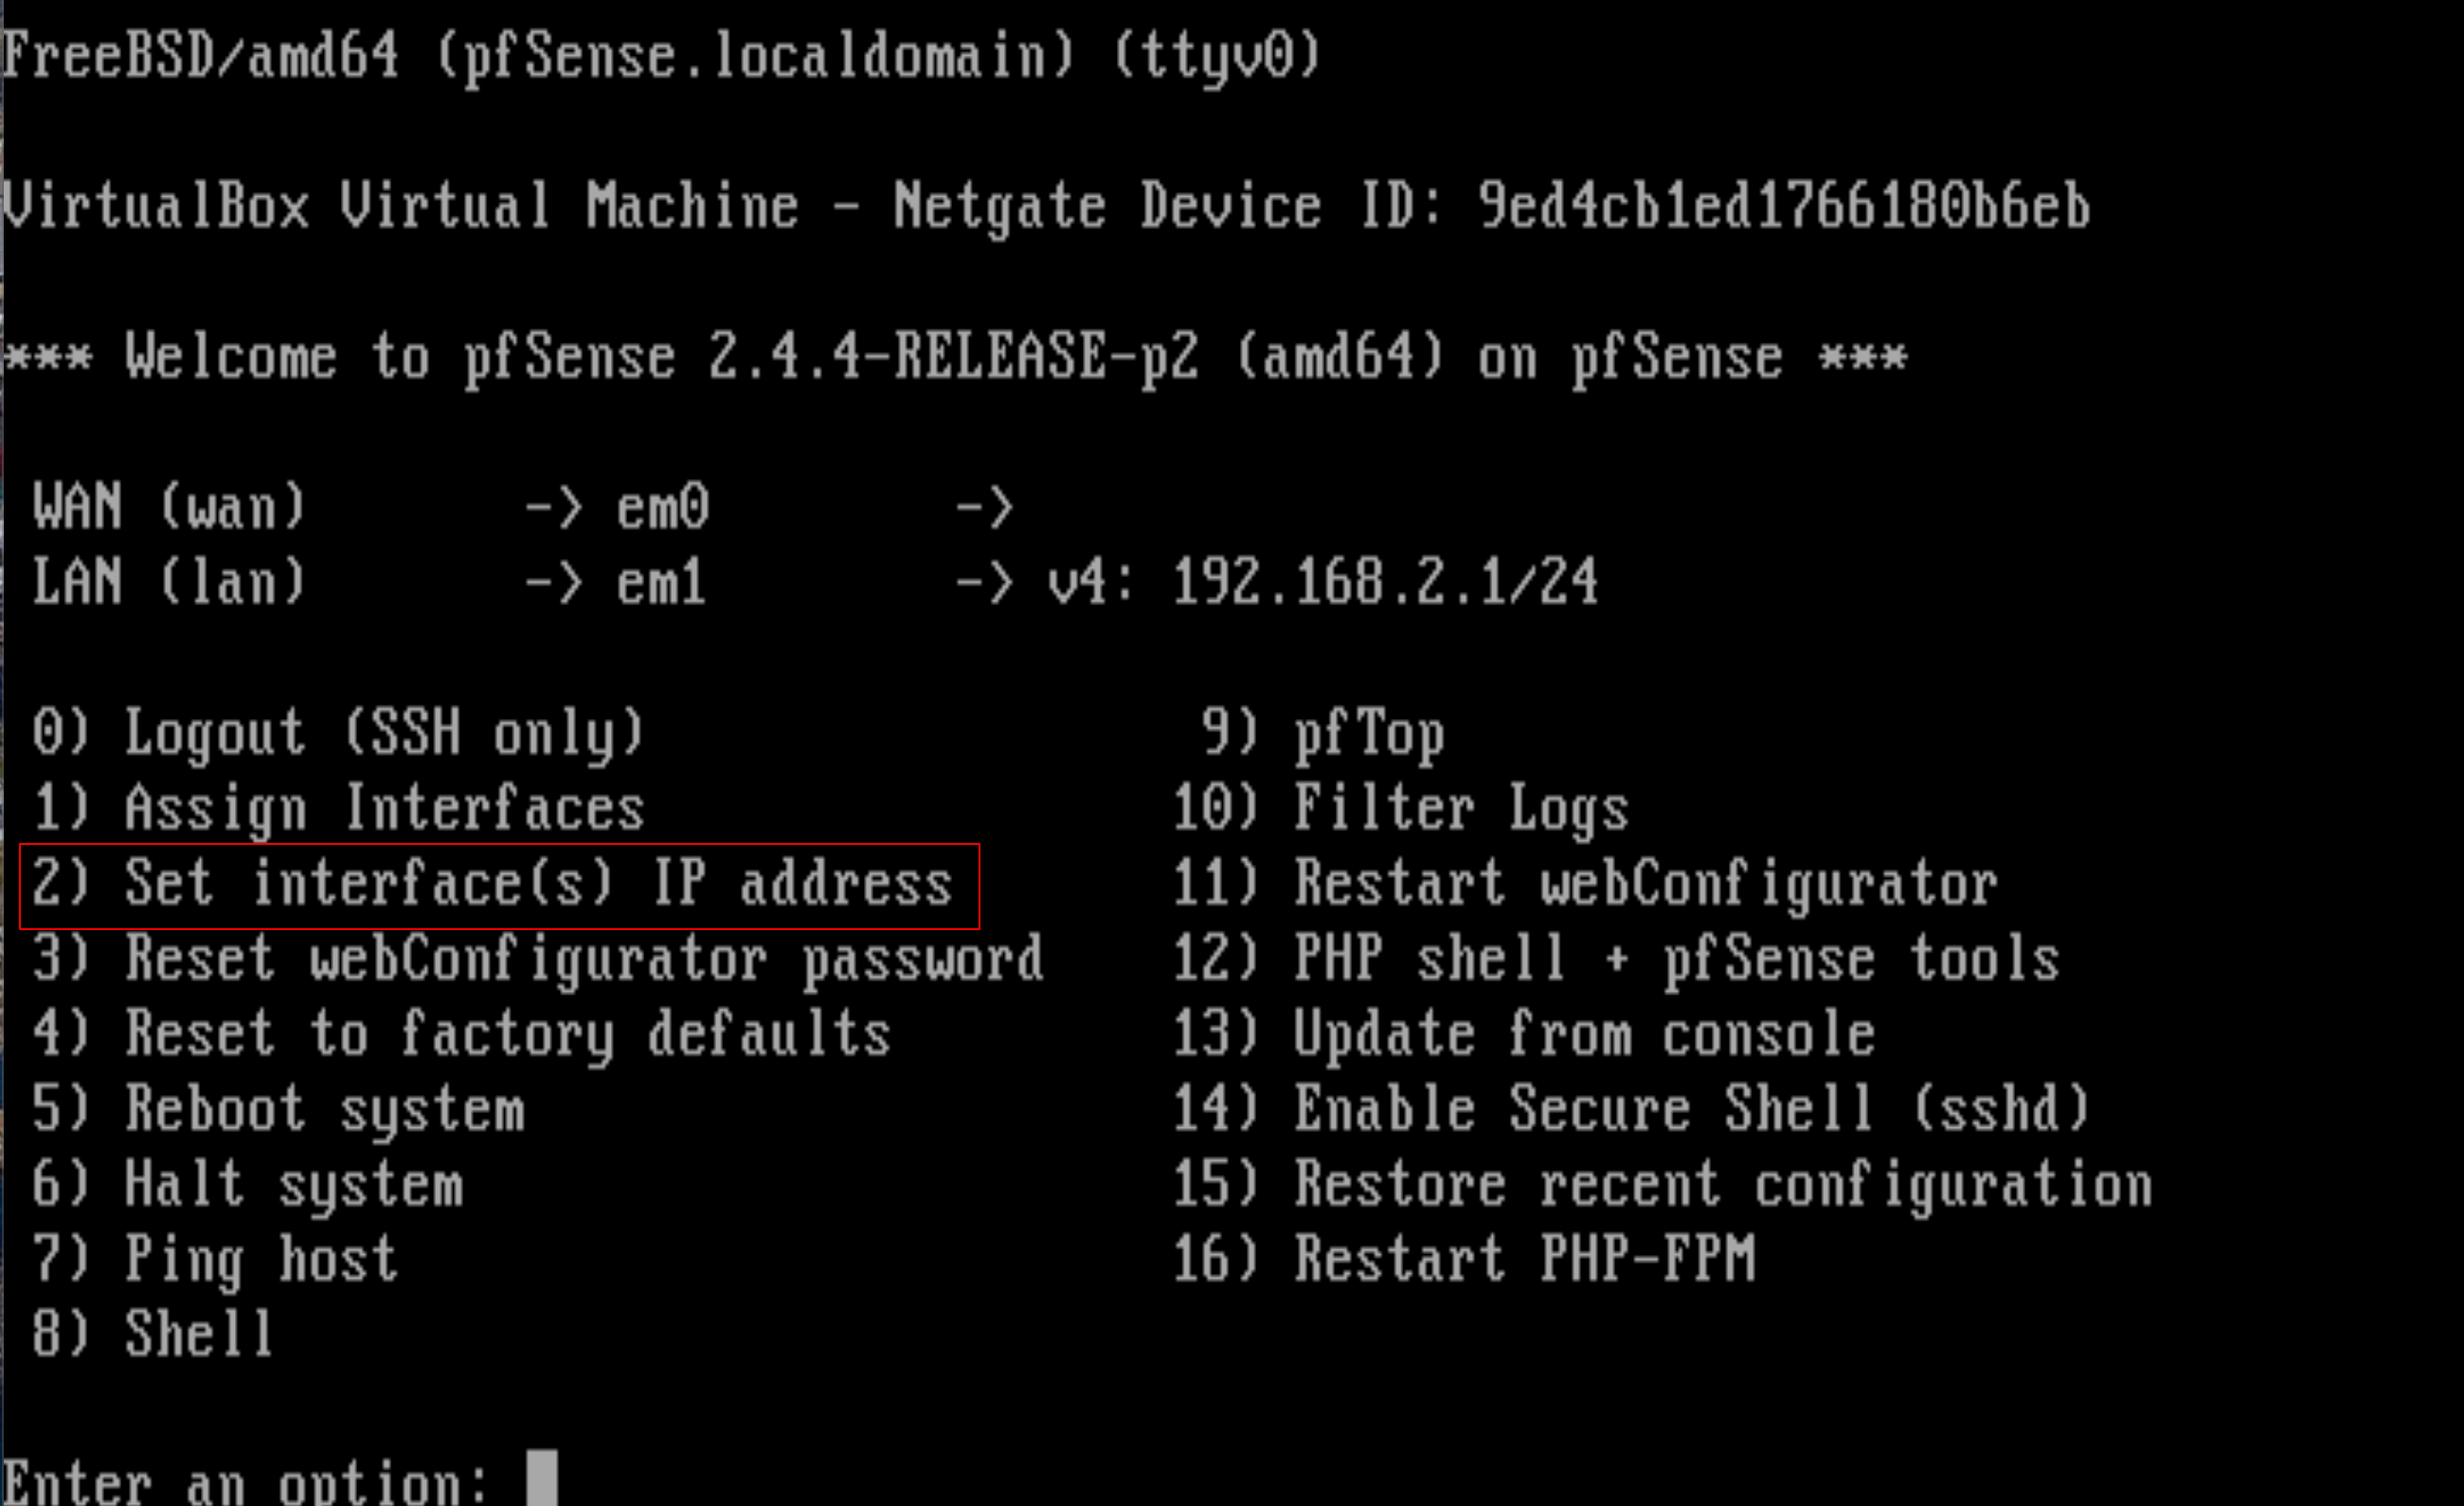
\includegraphics[scale=0.5]{Pfsense_Screeshots/15.png}
		\caption{Sélection de l'option de configuration des adresses IP de Pfsense}
		\label{Pfsense_Screeshots/15}
	\end{center}
\end{figure}
\FloatBarrier    

\newpage
Taper \textbf{1}, puis \textbf{y}, et \textbf{n}. Appuyer sur \textbf{Entrée}, puis ré-entrer \textbf{n}. Appuyer une dernière fois sur \textbf{Entrée} :
\begin{figure}[h!]
	\begin{center}
		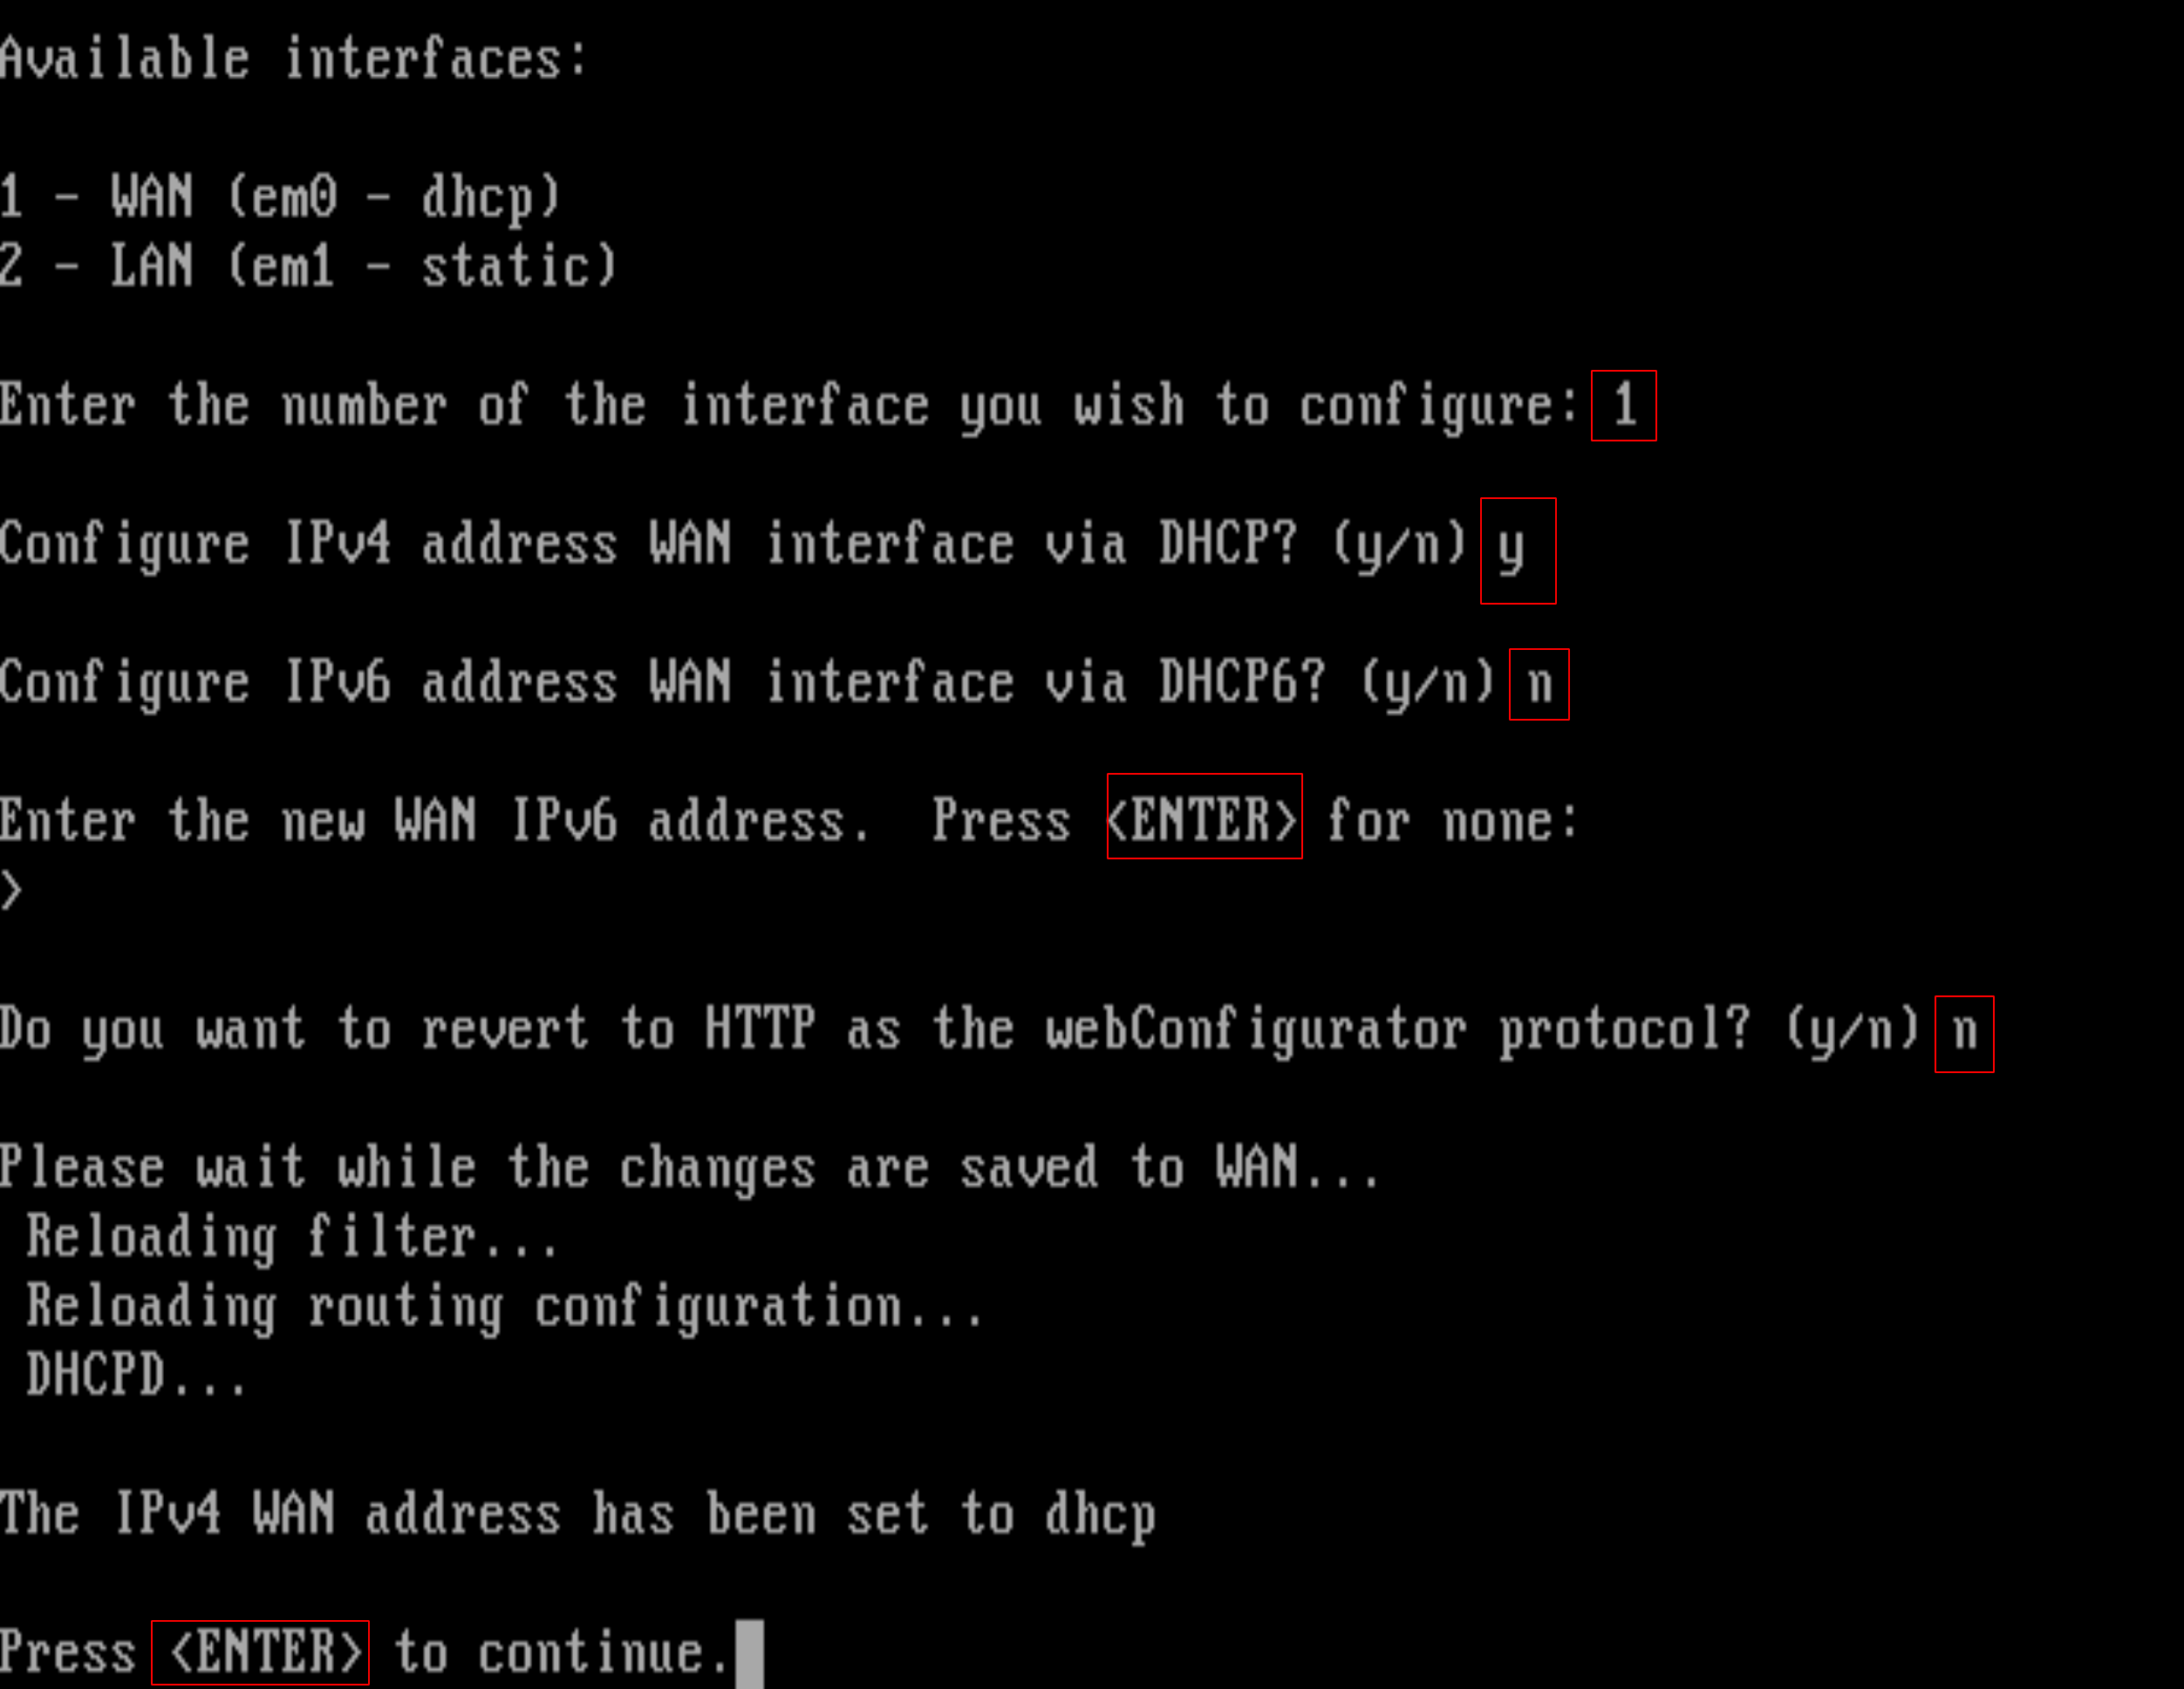
\includegraphics[scale=0.5]{Pfsense_Screeshots/16.png}
		\caption{Configuration des adresses IP de l'interface réseau WAN de Pfsense}
		\label{Pfsense_Screeshots/16}
	\end{center}
\end{figure}
\FloatBarrier

\newpage
Sélectionner l'option de configuration des interfaces IP, en tapant \textbf{2}, puis appuyer sur la touche \textbf{Entrée} :
\begin{figure}[h!]
	\begin{center}
		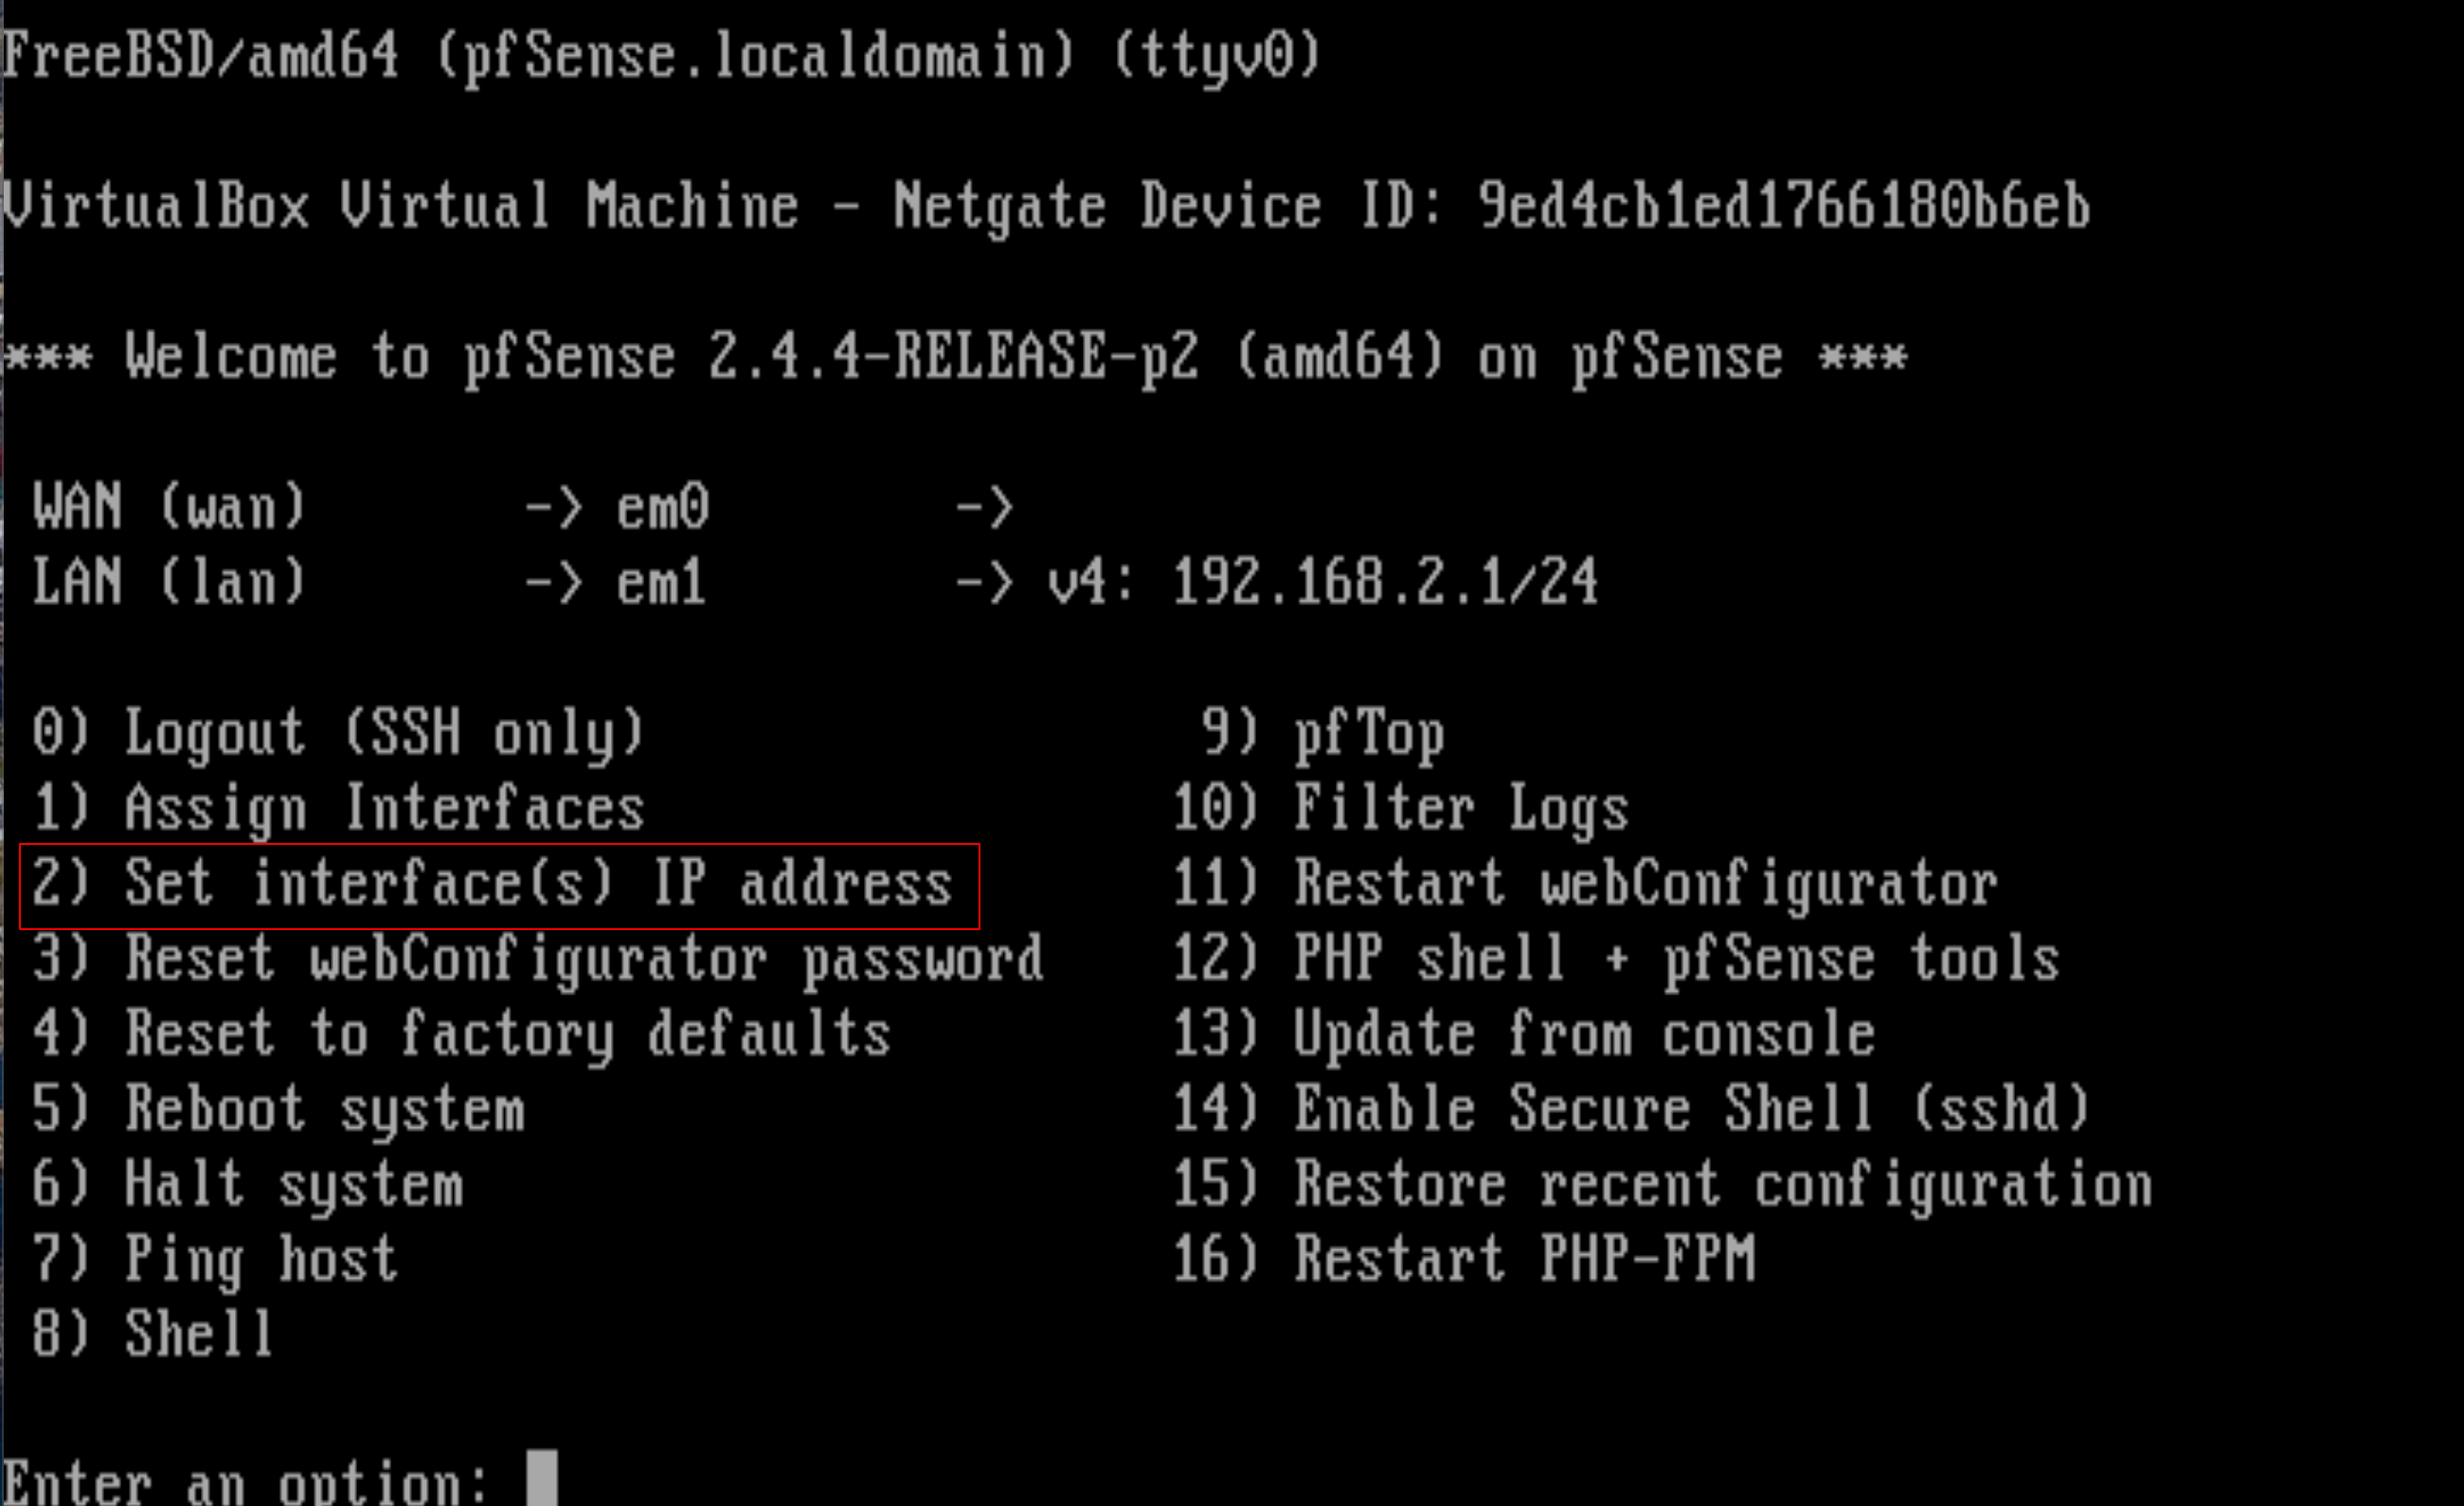
\includegraphics[scale=0.5]{Pfsense_Screeshots/15.png}
		\caption{Sélection de l'option de configuration des adresses IP de Pfsense}
		\label{Pfsense_Screeshots/15}
	\end{center}
\end{figure}
\FloatBarrier

\newpage
Taper \textbf{2}. Entrer l'adresse IP : 192.168.2.1. Taper \textbf{24}, puis appuyer deux fois sur la touche \textbf{Entrée}. Taper \textbf{n} aux deux dernières questions :
\begin{figure}[h!]
	\begin{center}
		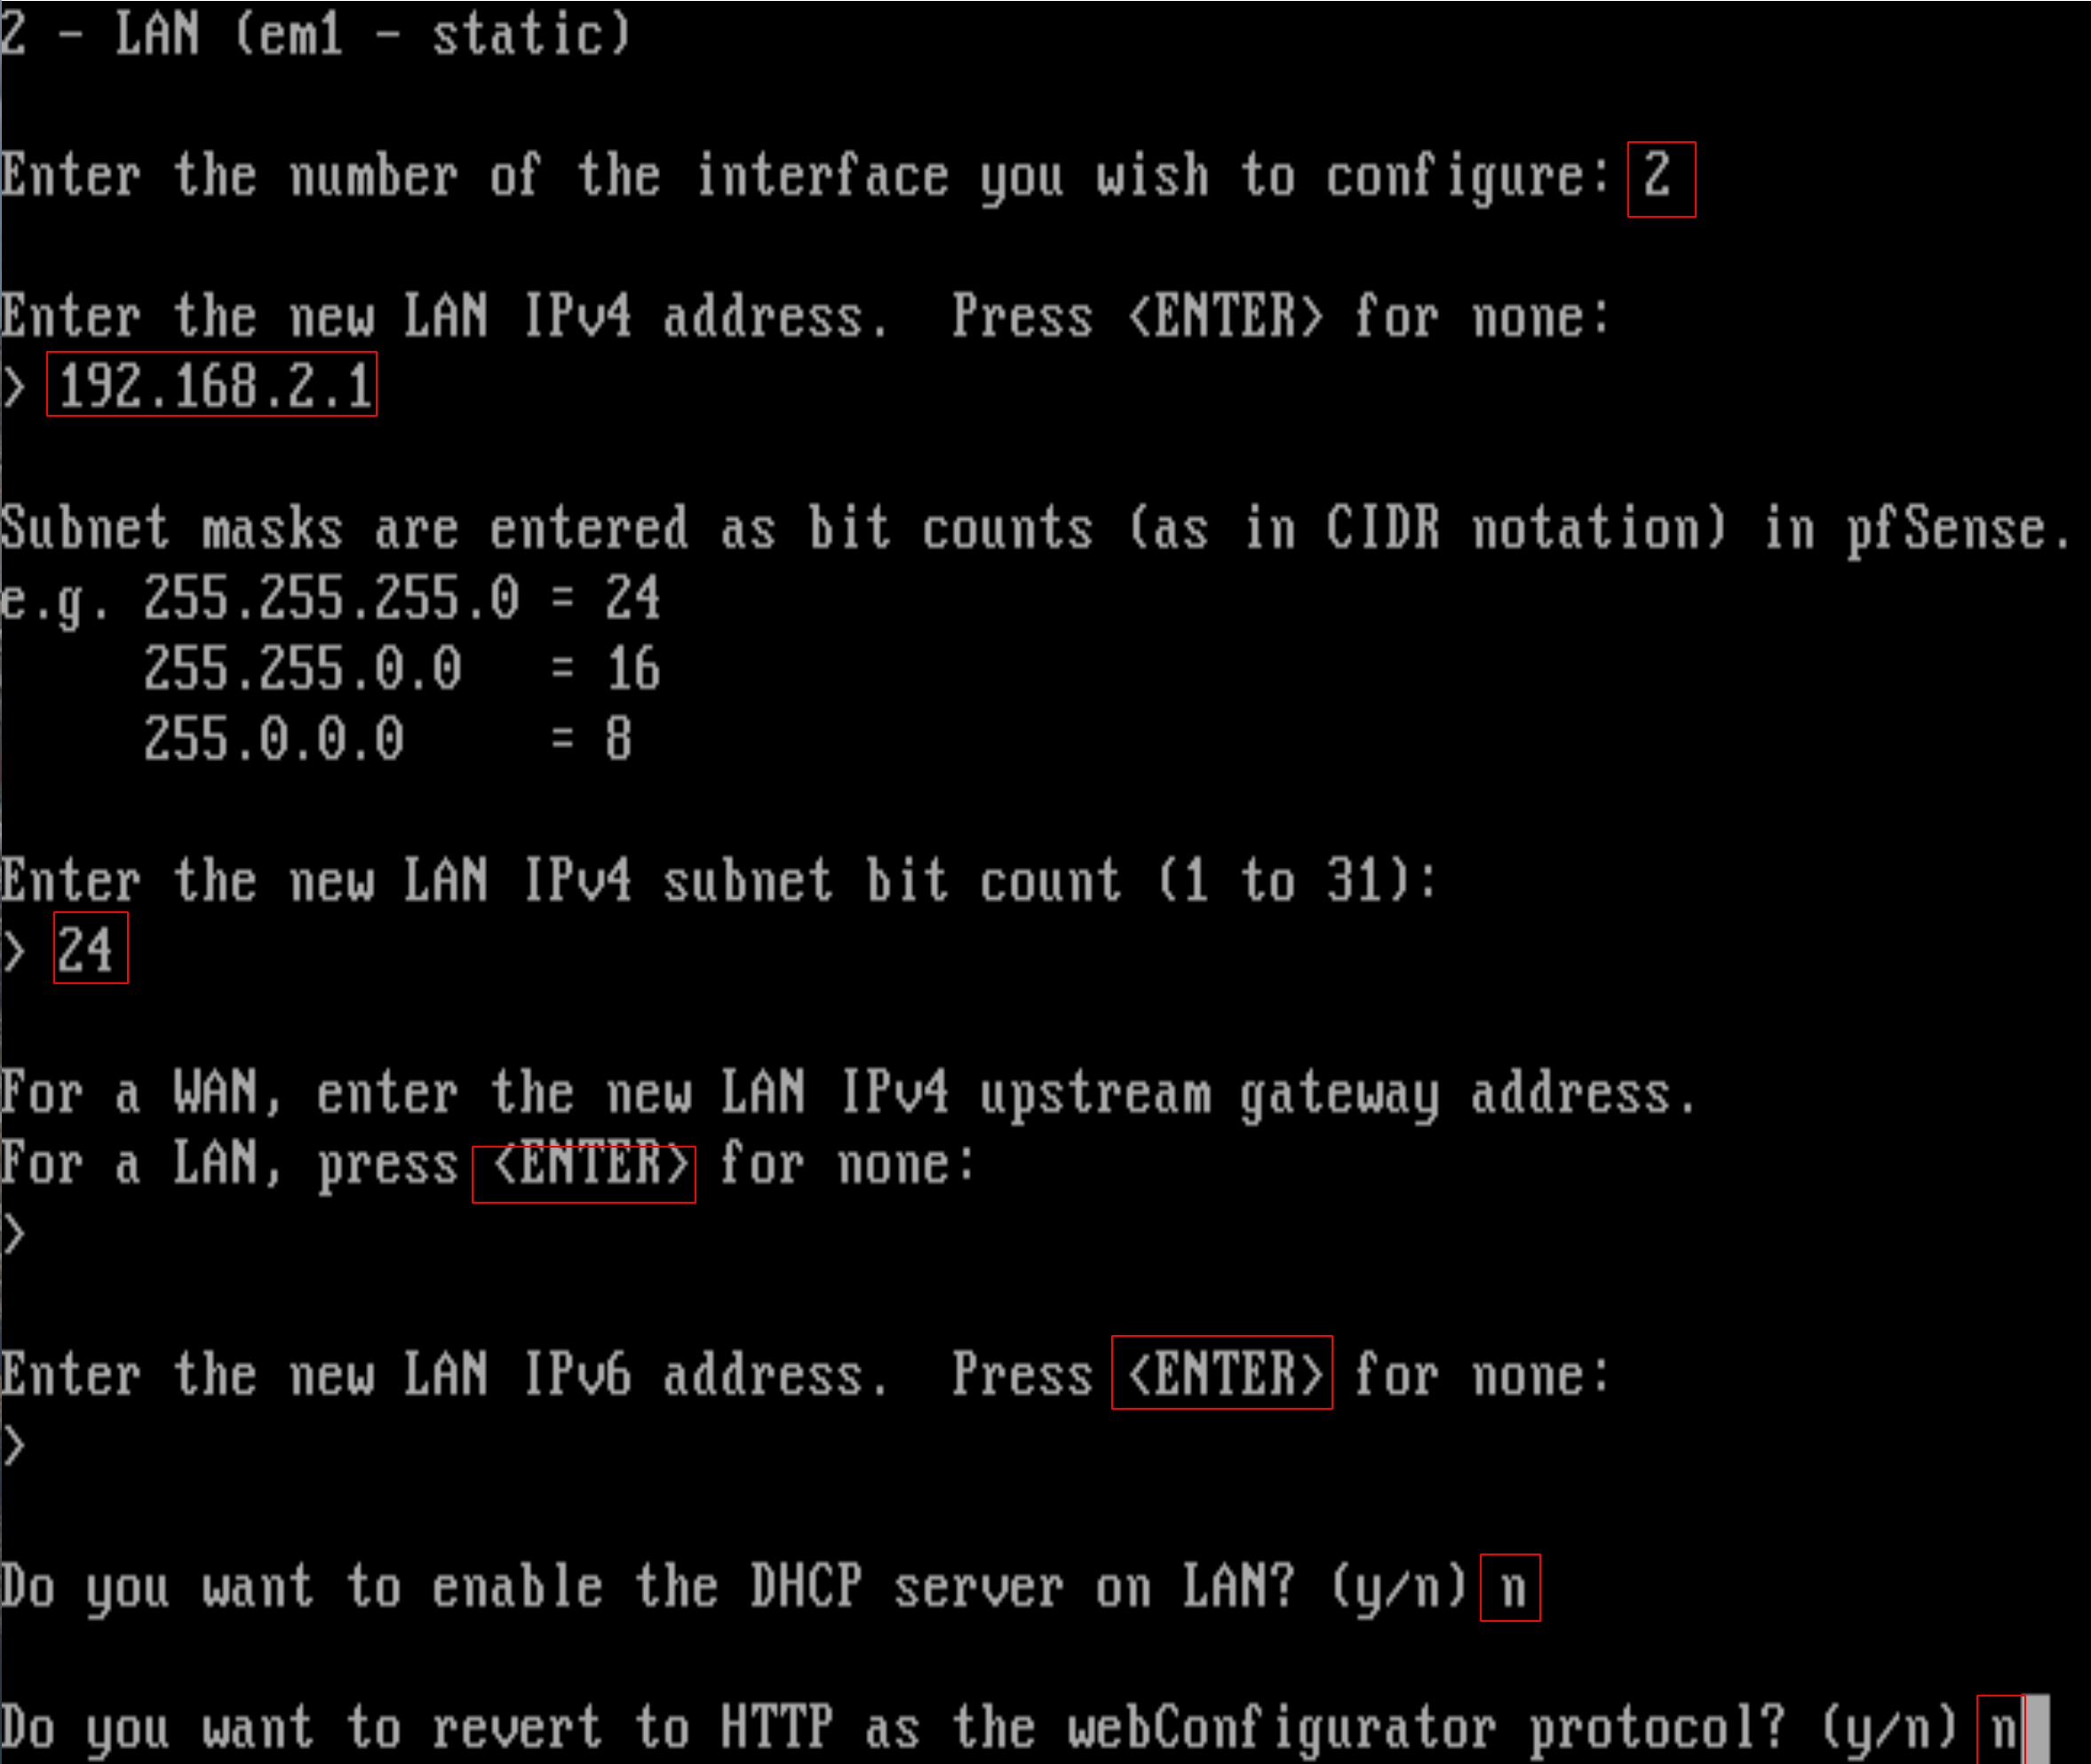
\includegraphics[scale=0.5]{Pfsense_Screeshots/17.png}
		\caption{Configuration des adresses IP de l'interface réseau LAN de Pfsense}
		\label{Pfsense_Screeshots/17}
	\end{center}
\end{figure}
\FloatBarrier    

\newpage
Vérifier le bon paramétrage de Pfsense avec la figure suivante :
\begin{figure}[h!]
	\begin{center}
		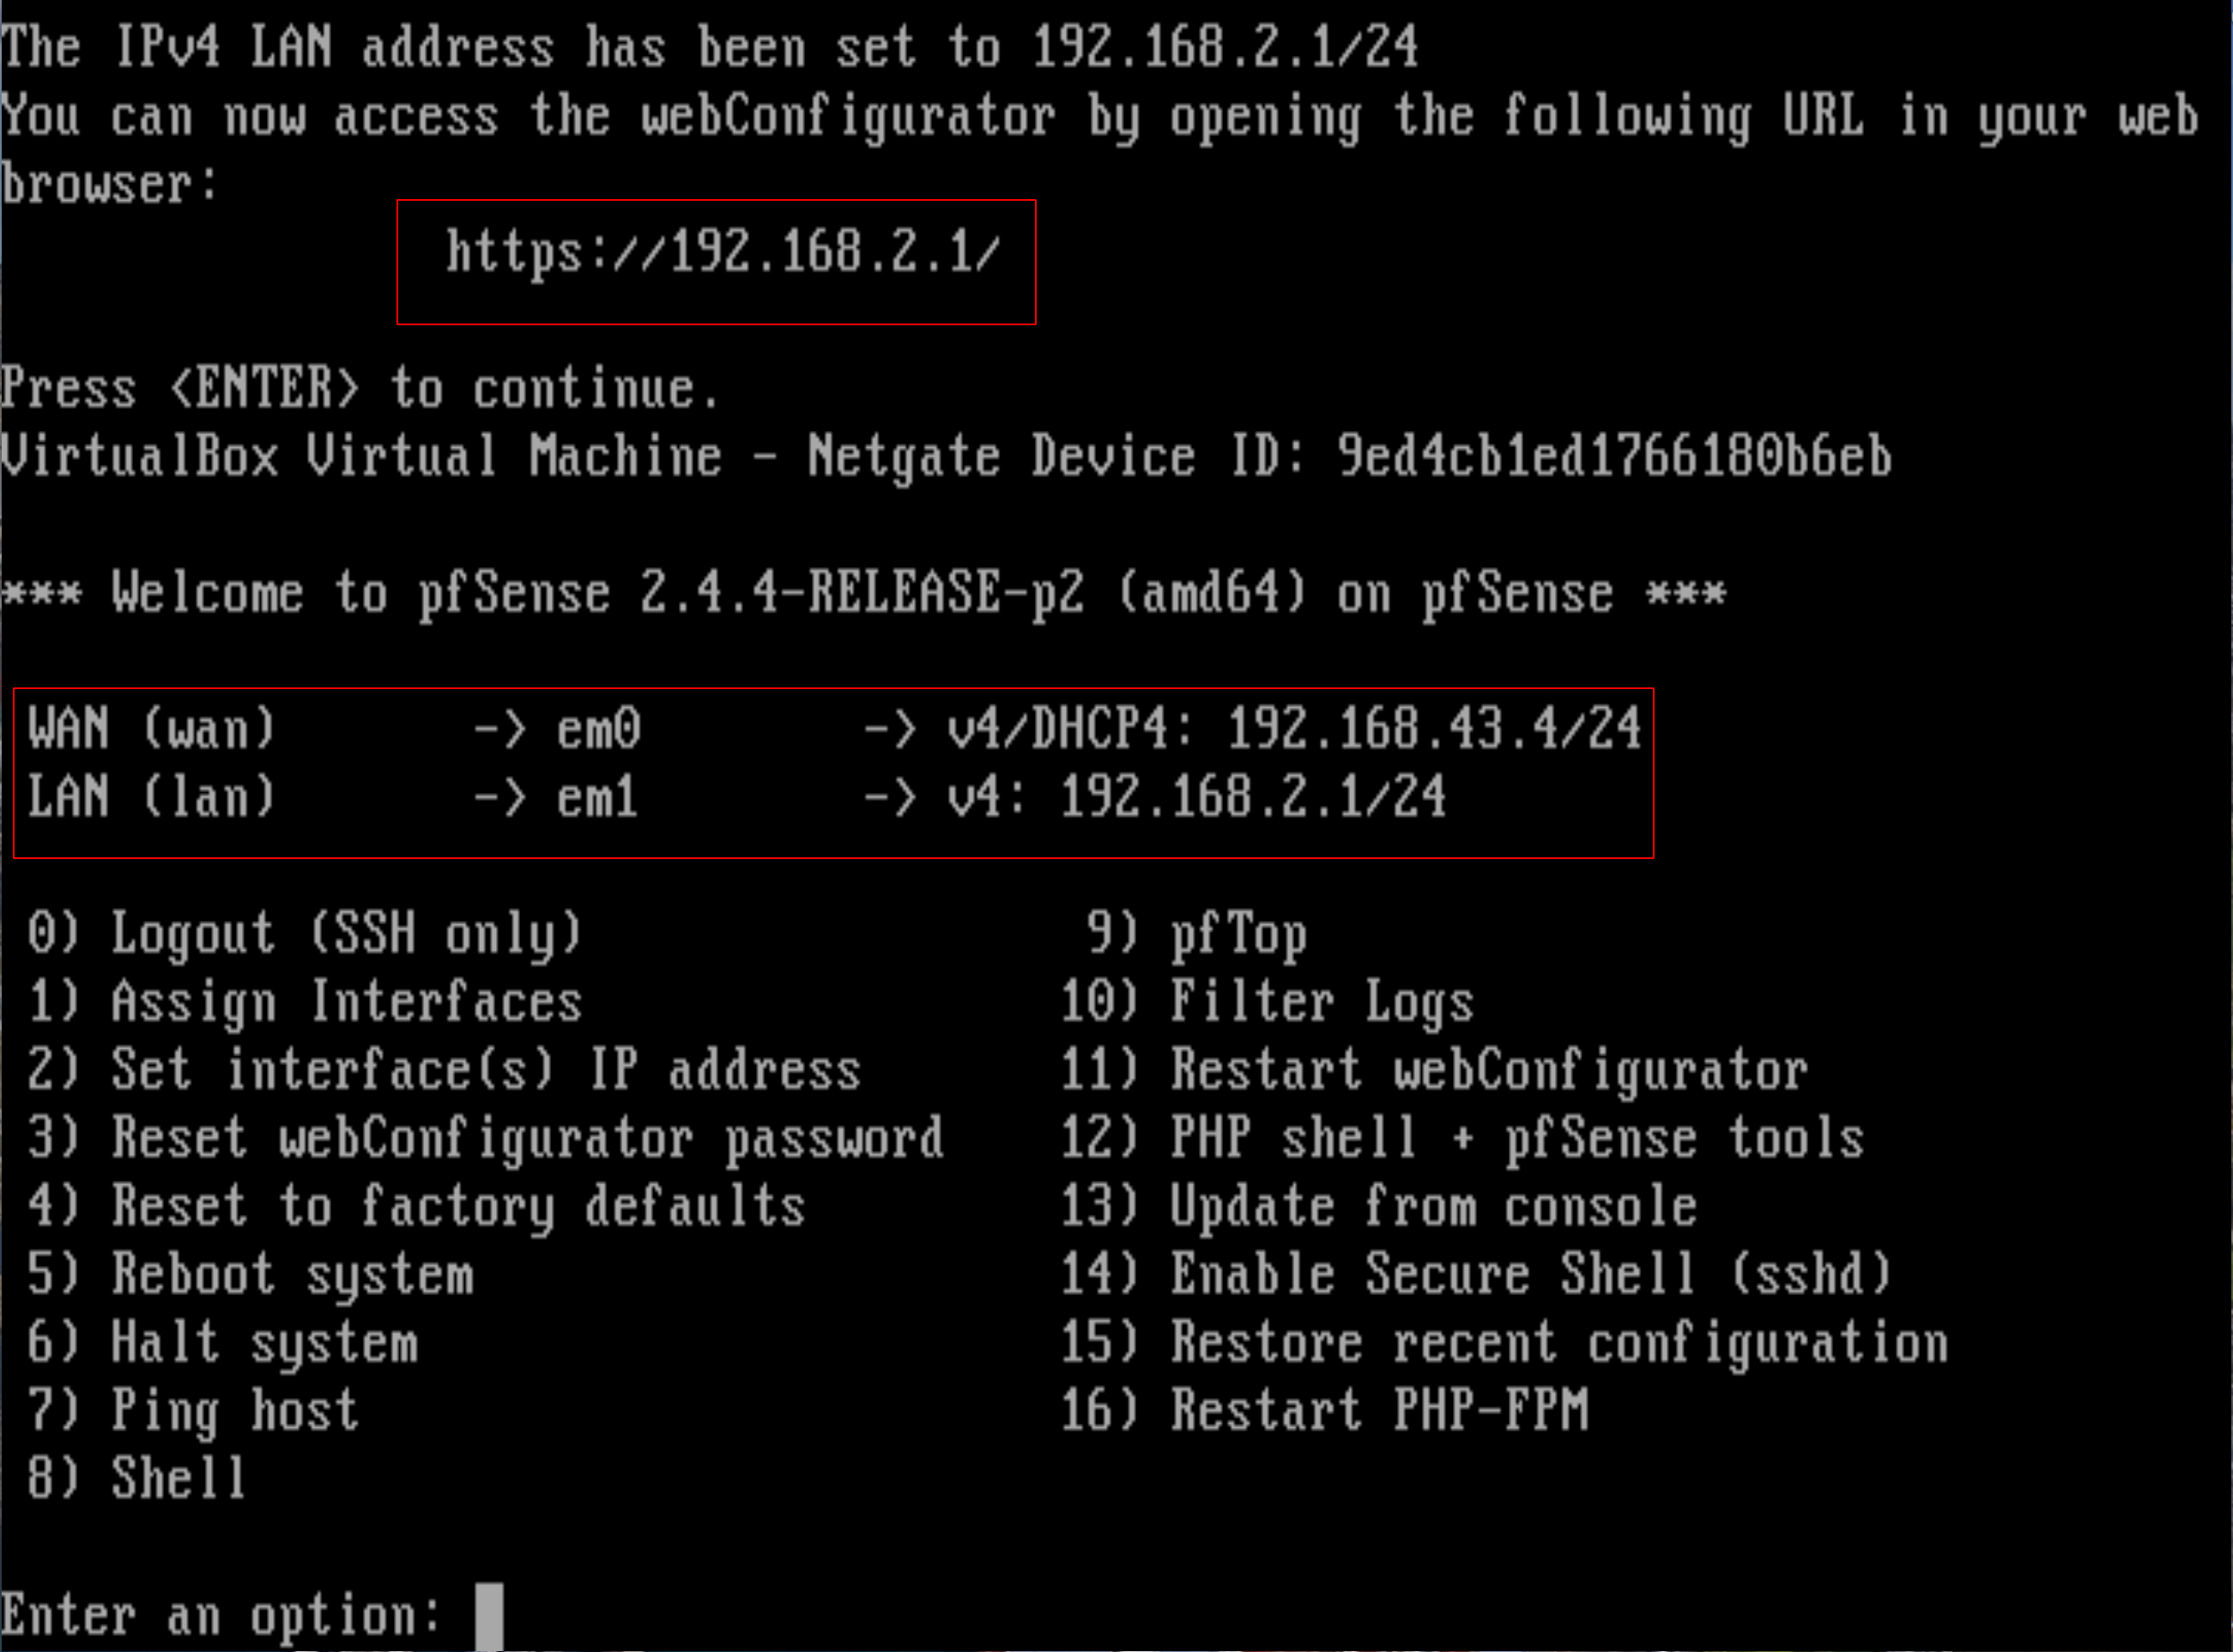
\includegraphics[scale=0.5]{Pfsense_Screeshots/18.png}
		\caption{Vérification du paramétrage de Pfsense}
		\label{Pfsense_Screeshots/18}
	\end{center}
\end{figure}
\FloatBarrier

\newpage
\subsection{Configuration des règles Pfsense}

Démarrer la machine virtuelle Windows Server 2012. Se connecter sur la machine Windows Server 2012 avec le compte administrateur et le mot de passe définit à l'installation :
\begin{figure}[h!]
	\begin{center}
		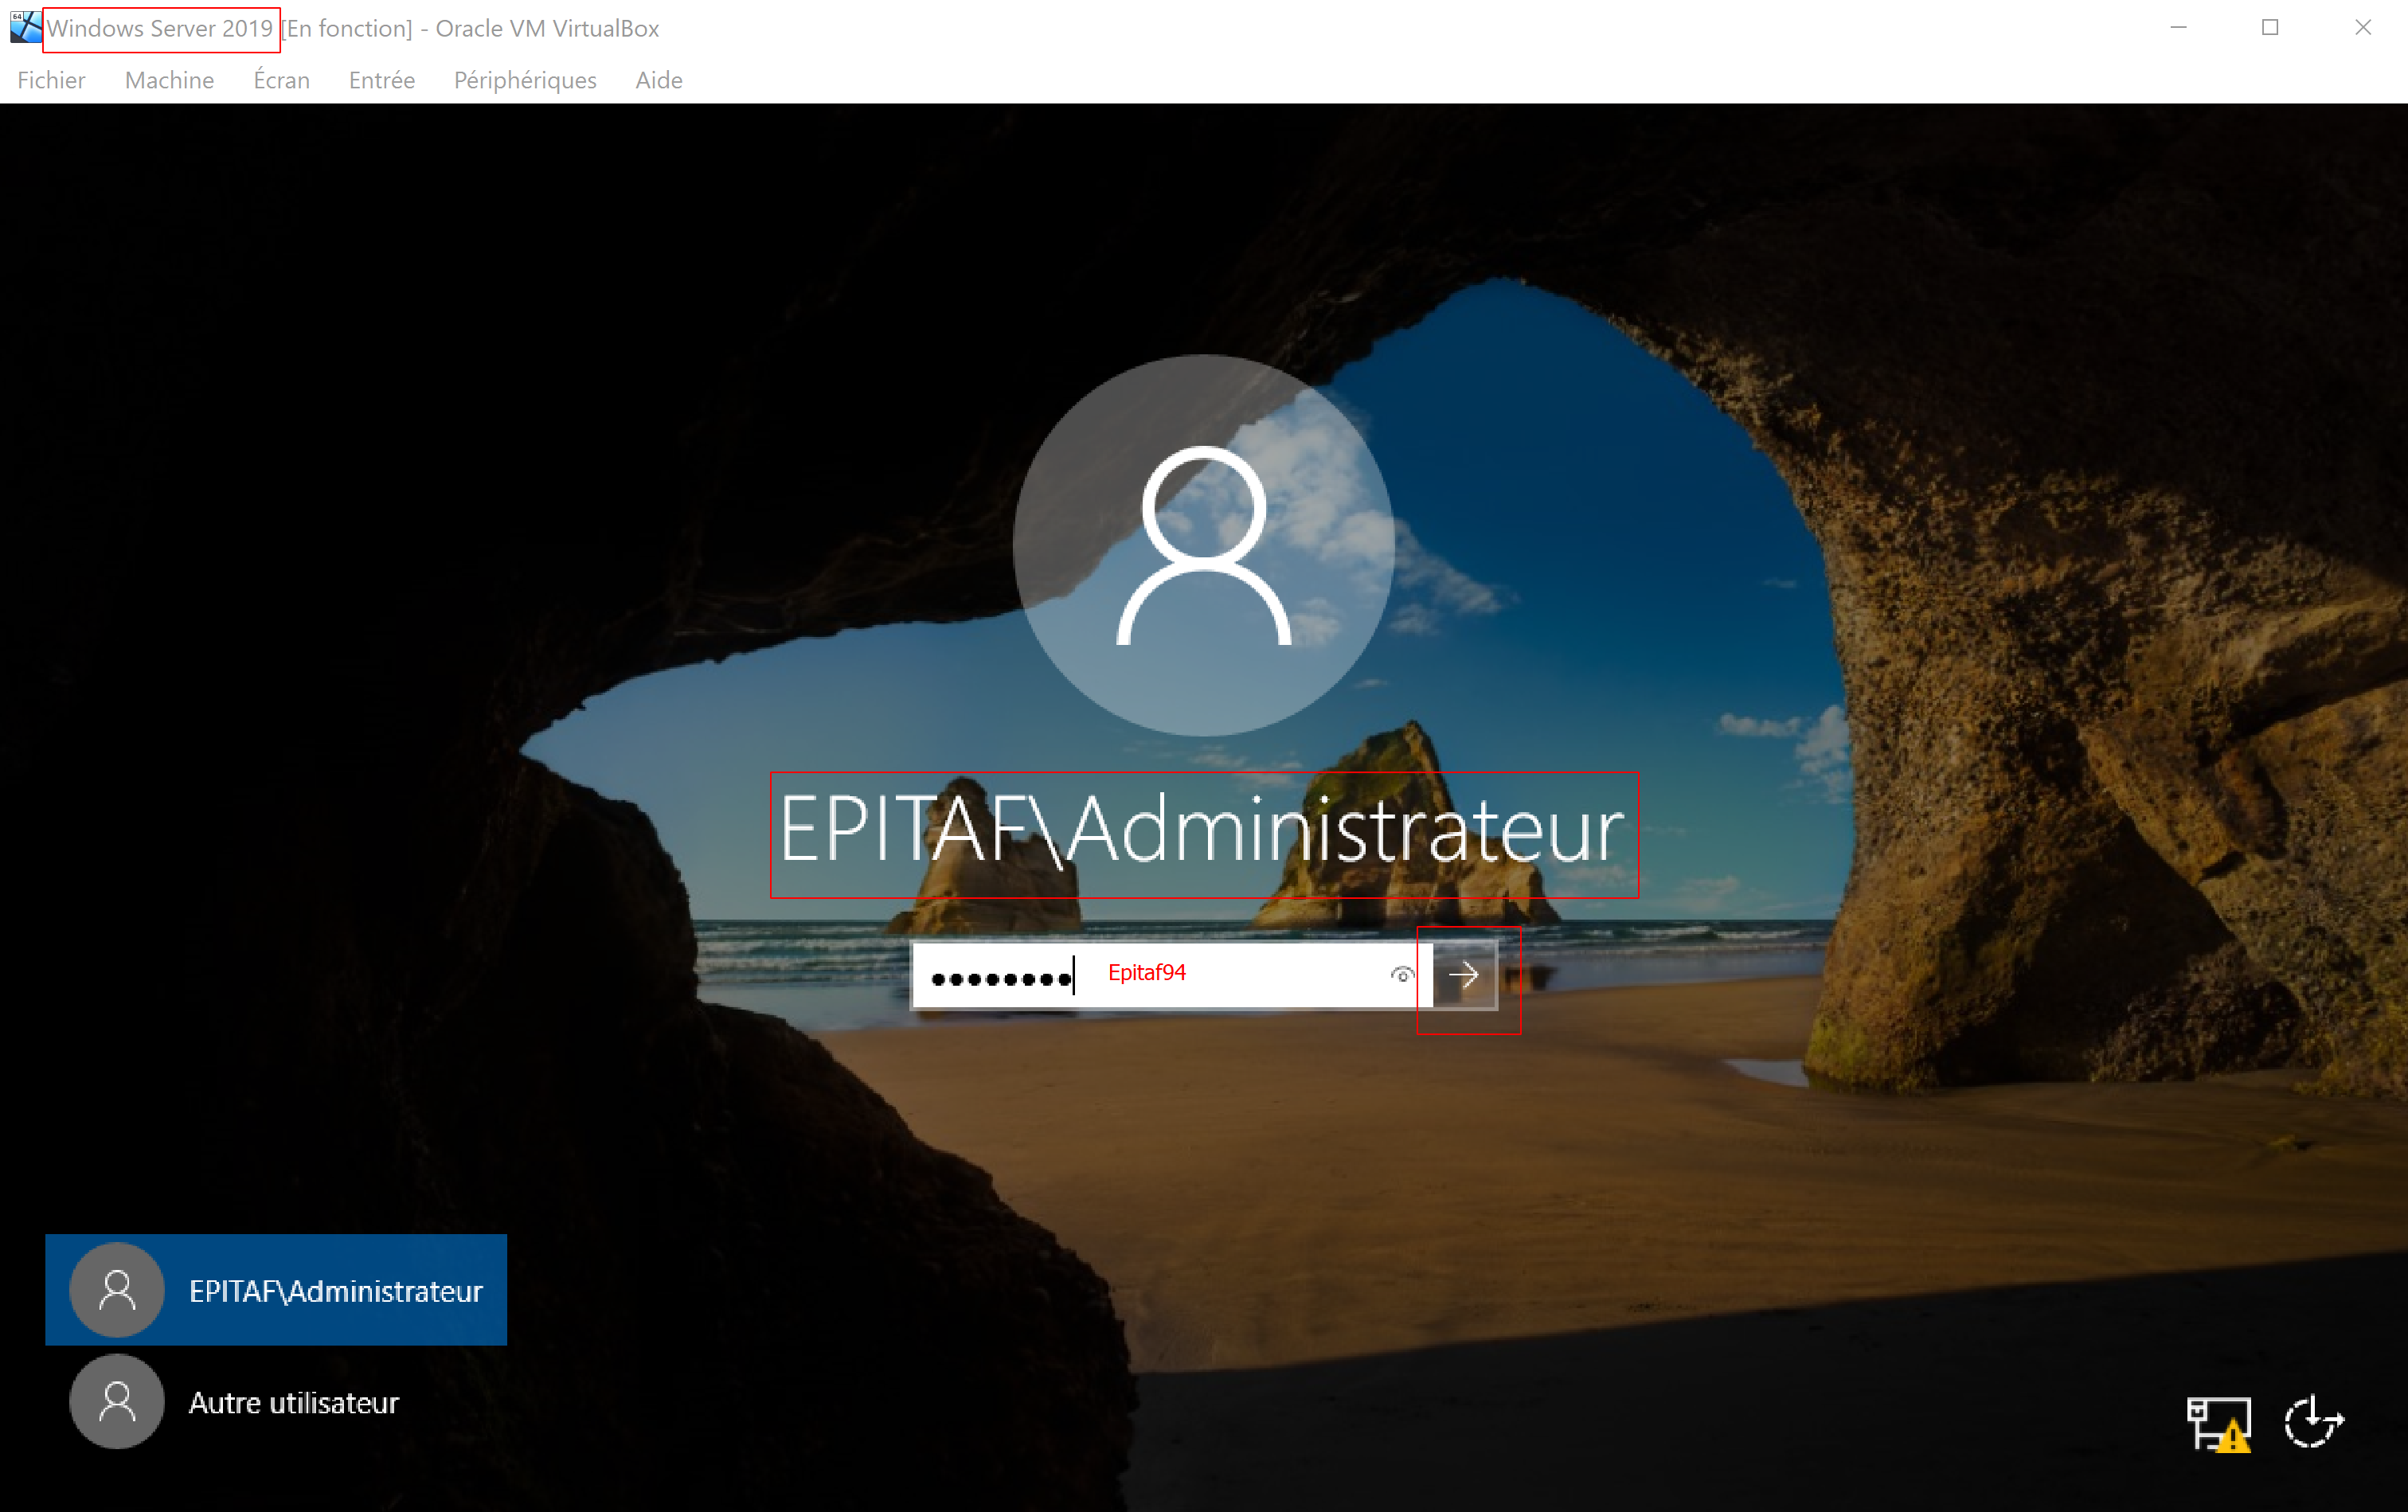
\includegraphics[scale=0.5]{Pfsense_Screeshots/19.png}
		\caption{Connexion à Windows Server}
		\label{Pfsense_Screeshots/19}
	\end{center}
\end{figure}
\FloatBarrier

\newpage
Ouvrir Internet Explorer, et aller à l'adresse : 192.168.2.1. Se connecter avec les identifiants Pfsense par défaut. Changer le mot de passe de Pfsense :
\begin{figure}[h!]
	\begin{center}
		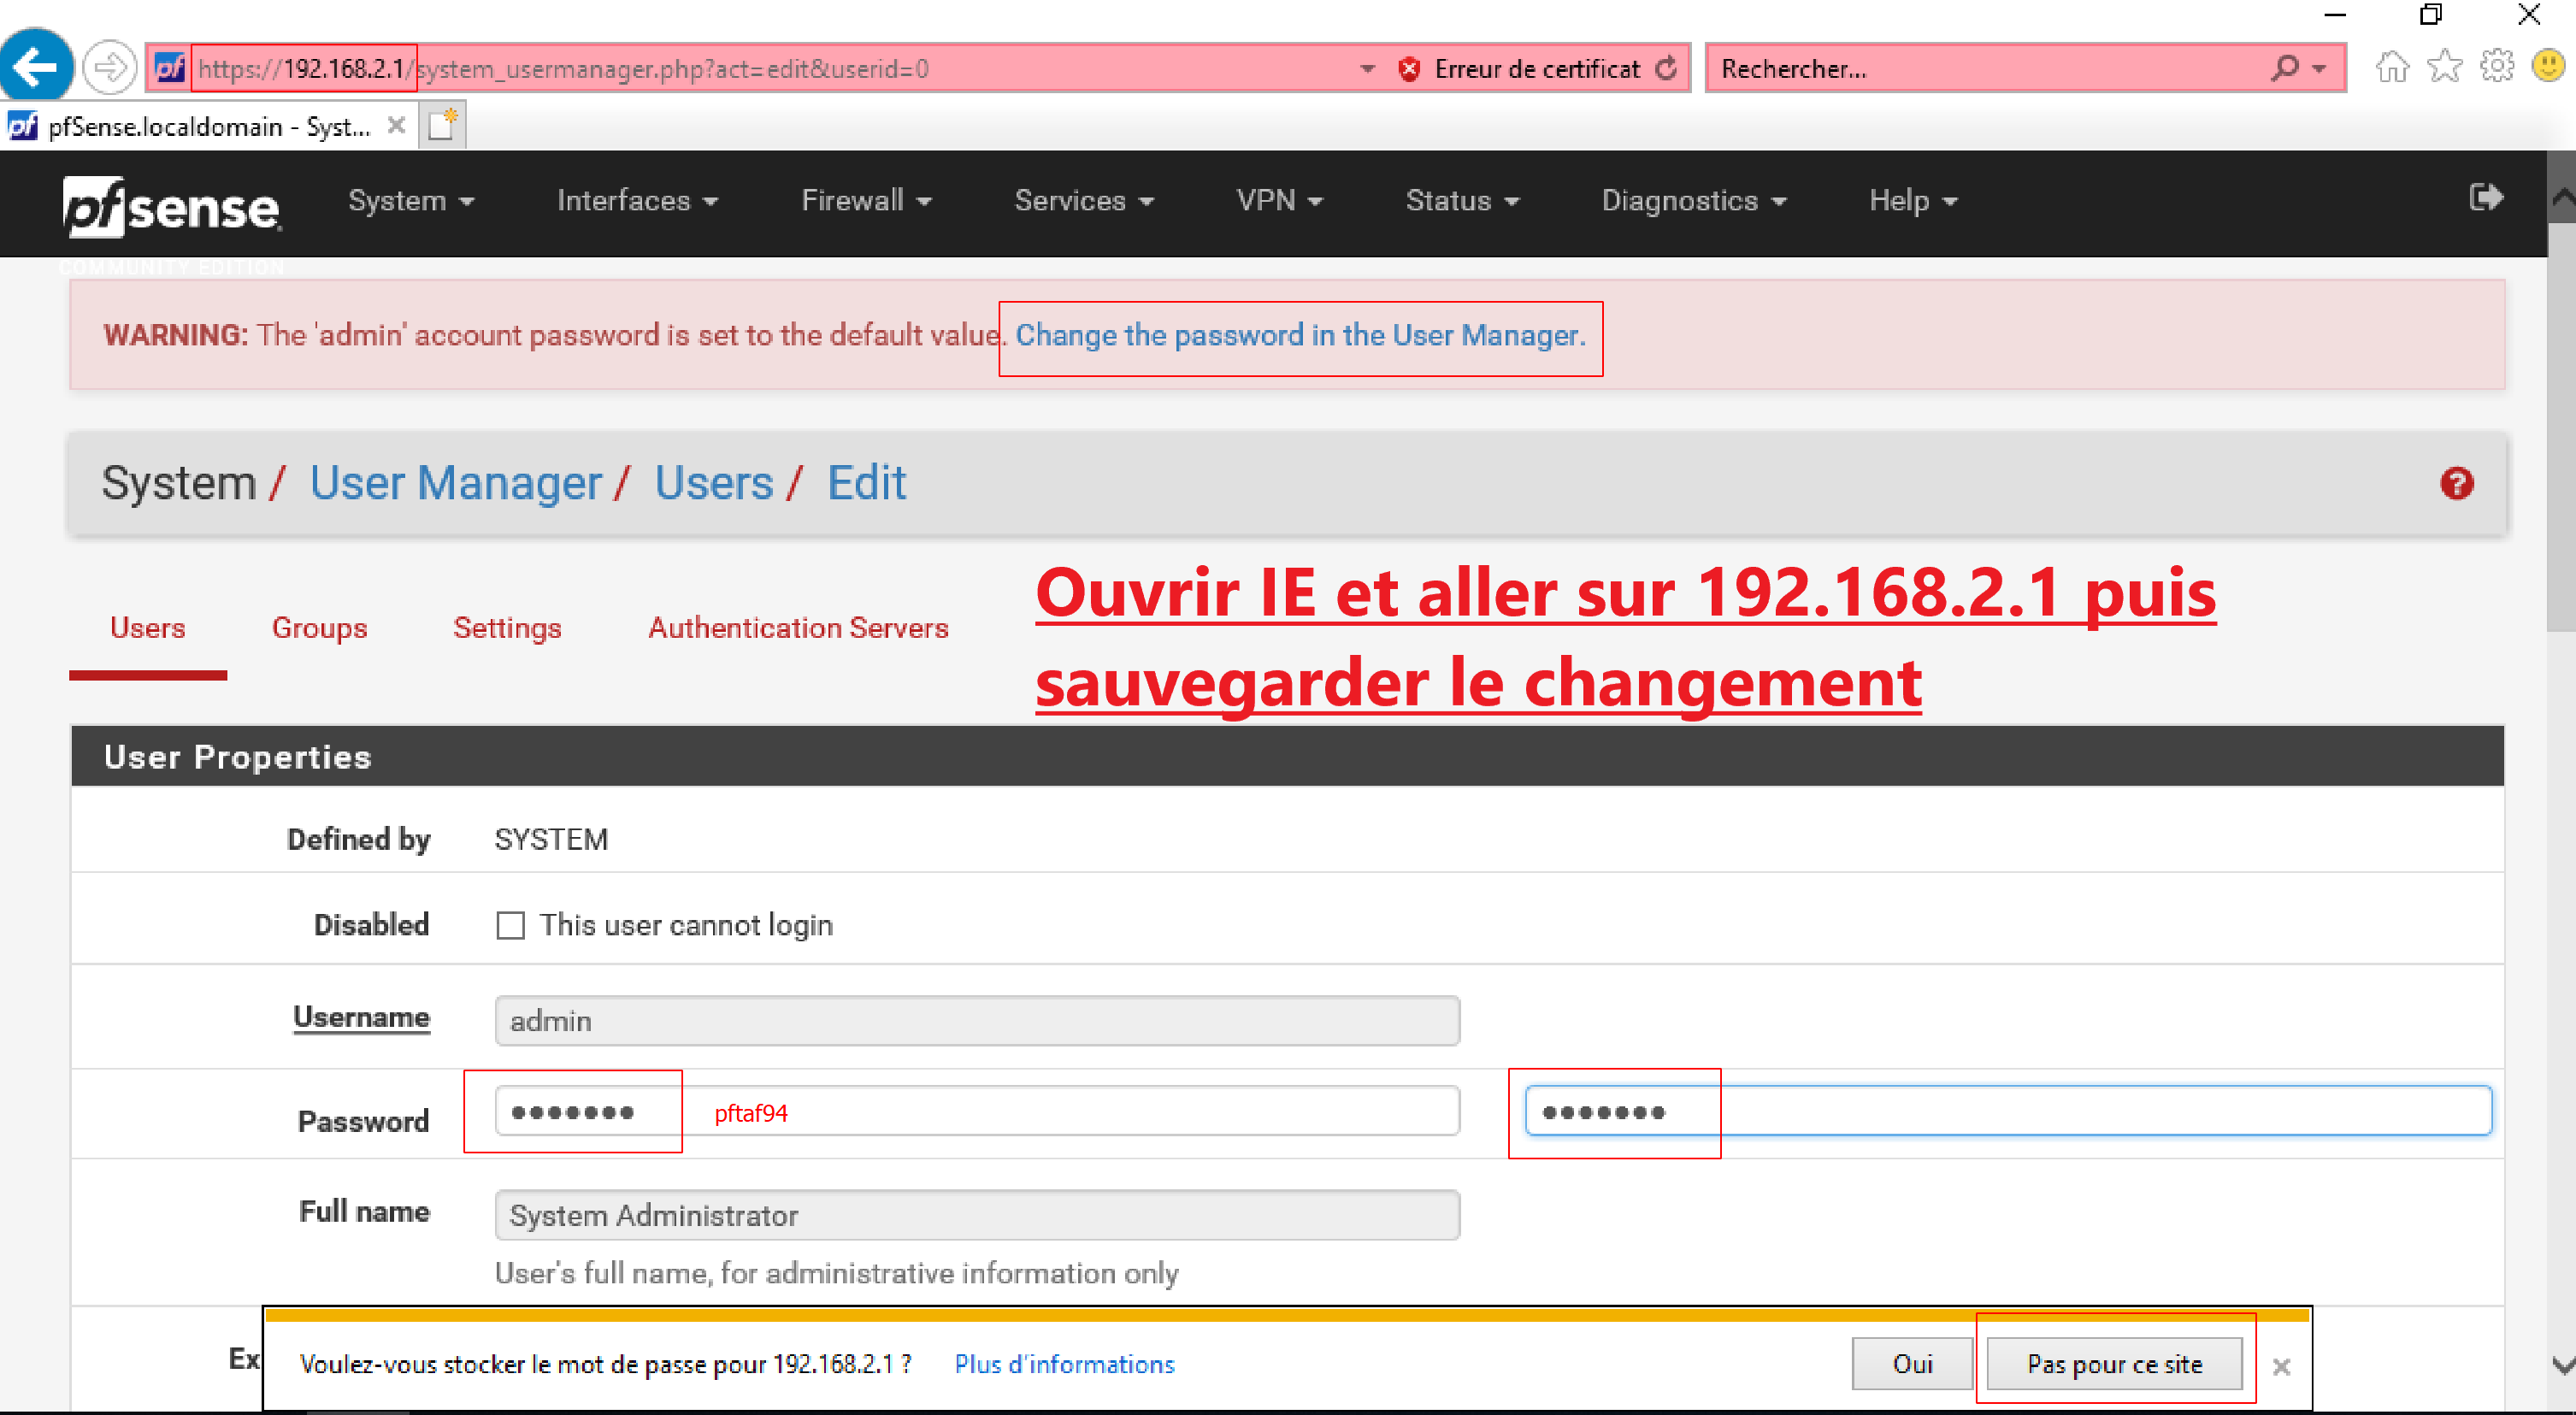
\includegraphics[scale=0.2]{Pfsense_Screeshots/20.png}
		\caption{Accès et changement des accès de Pfsense sur Windows Server}
		\label{Pfsense_Screeshots/20}
	\end{center}
\end{figure}
\FloatBarrier    

Accéder à la page \texttt{Rules}, située dans \textbf{Firewall} :
\begin{figure}[h!]
	\begin{center}
		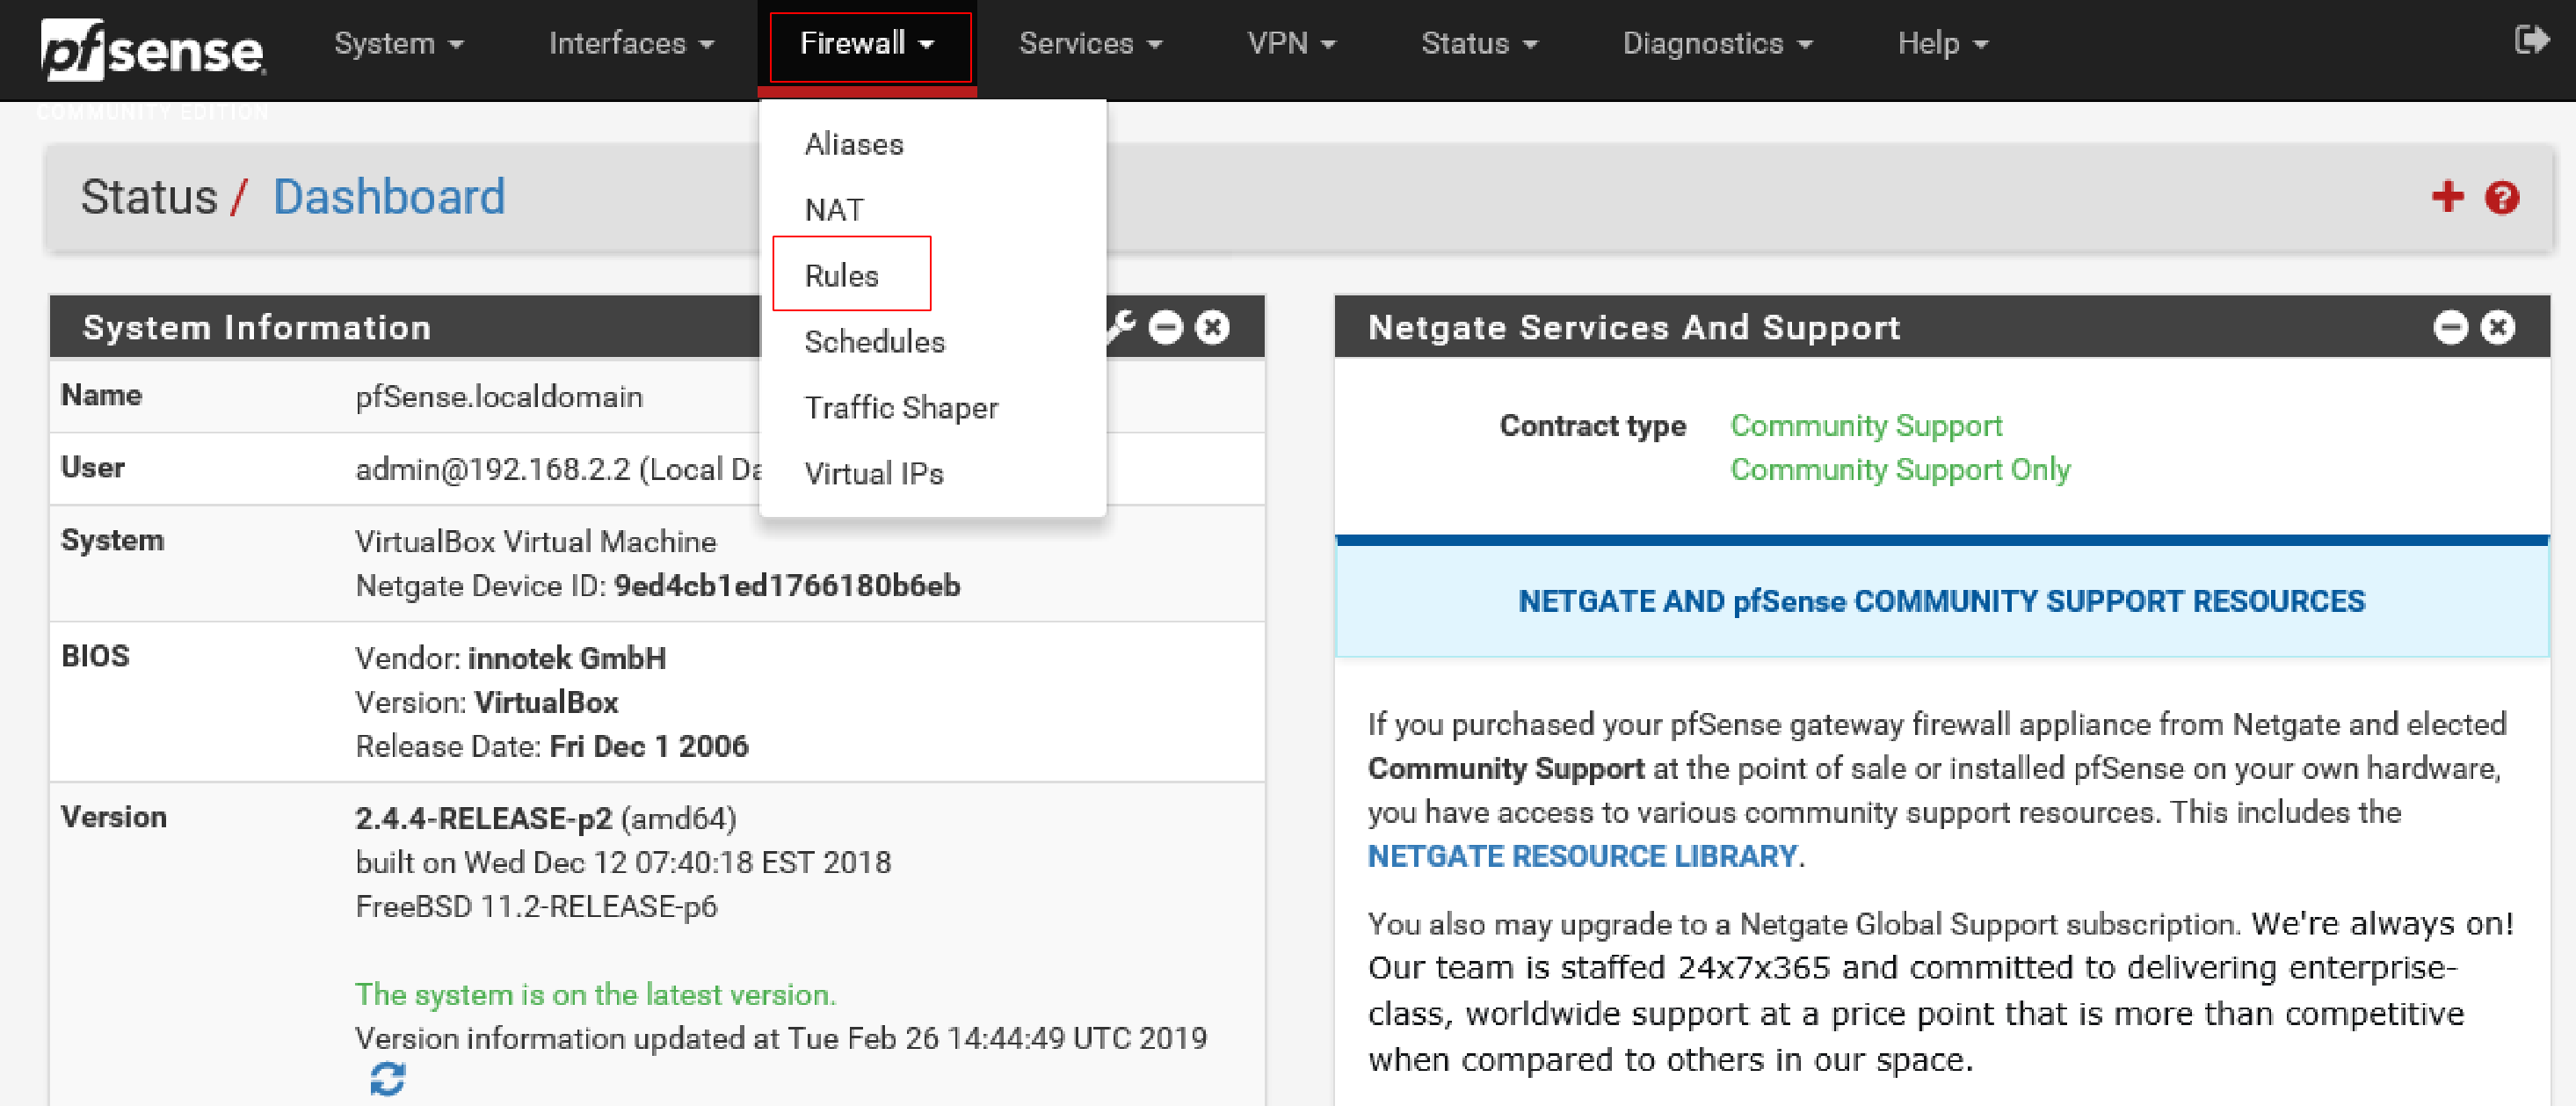
\includegraphics[scale=0.5]{Pfsense_Screeshots/21.png}
		\caption{Accès aux règles de Pfsense via Windows Server}
		\label{Pfsense_Screeshots/21}
	\end{center}
\end{figure}
\FloatBarrier

Aller dans la section \textit{LAN}. Les étapes de modification des règles Pfsense sont les suivantes :
\begin{itemize}
    \item Désactiver les deux règles existantes;
    \item Créer une règle filtrant les trames IPv4 TCP/UDP provenant de 192.168.2.2, sur le port 53 (DNS);
    \item Créer une règle filtrant les trames IPv4 TCP/UDP provenant de 192.168.2.0/24, sur le port 443 (HTTPS);
    \item Créer une règle filtrant les trames IPv4 TCP/UDP provenant de 192.168.2.0/24, sur le port 80 (HTTP).
\end{itemize}
Le résultat attendu est affiché sur la figure suivante :
\begin{figure}[h!]
	\begin{center}
		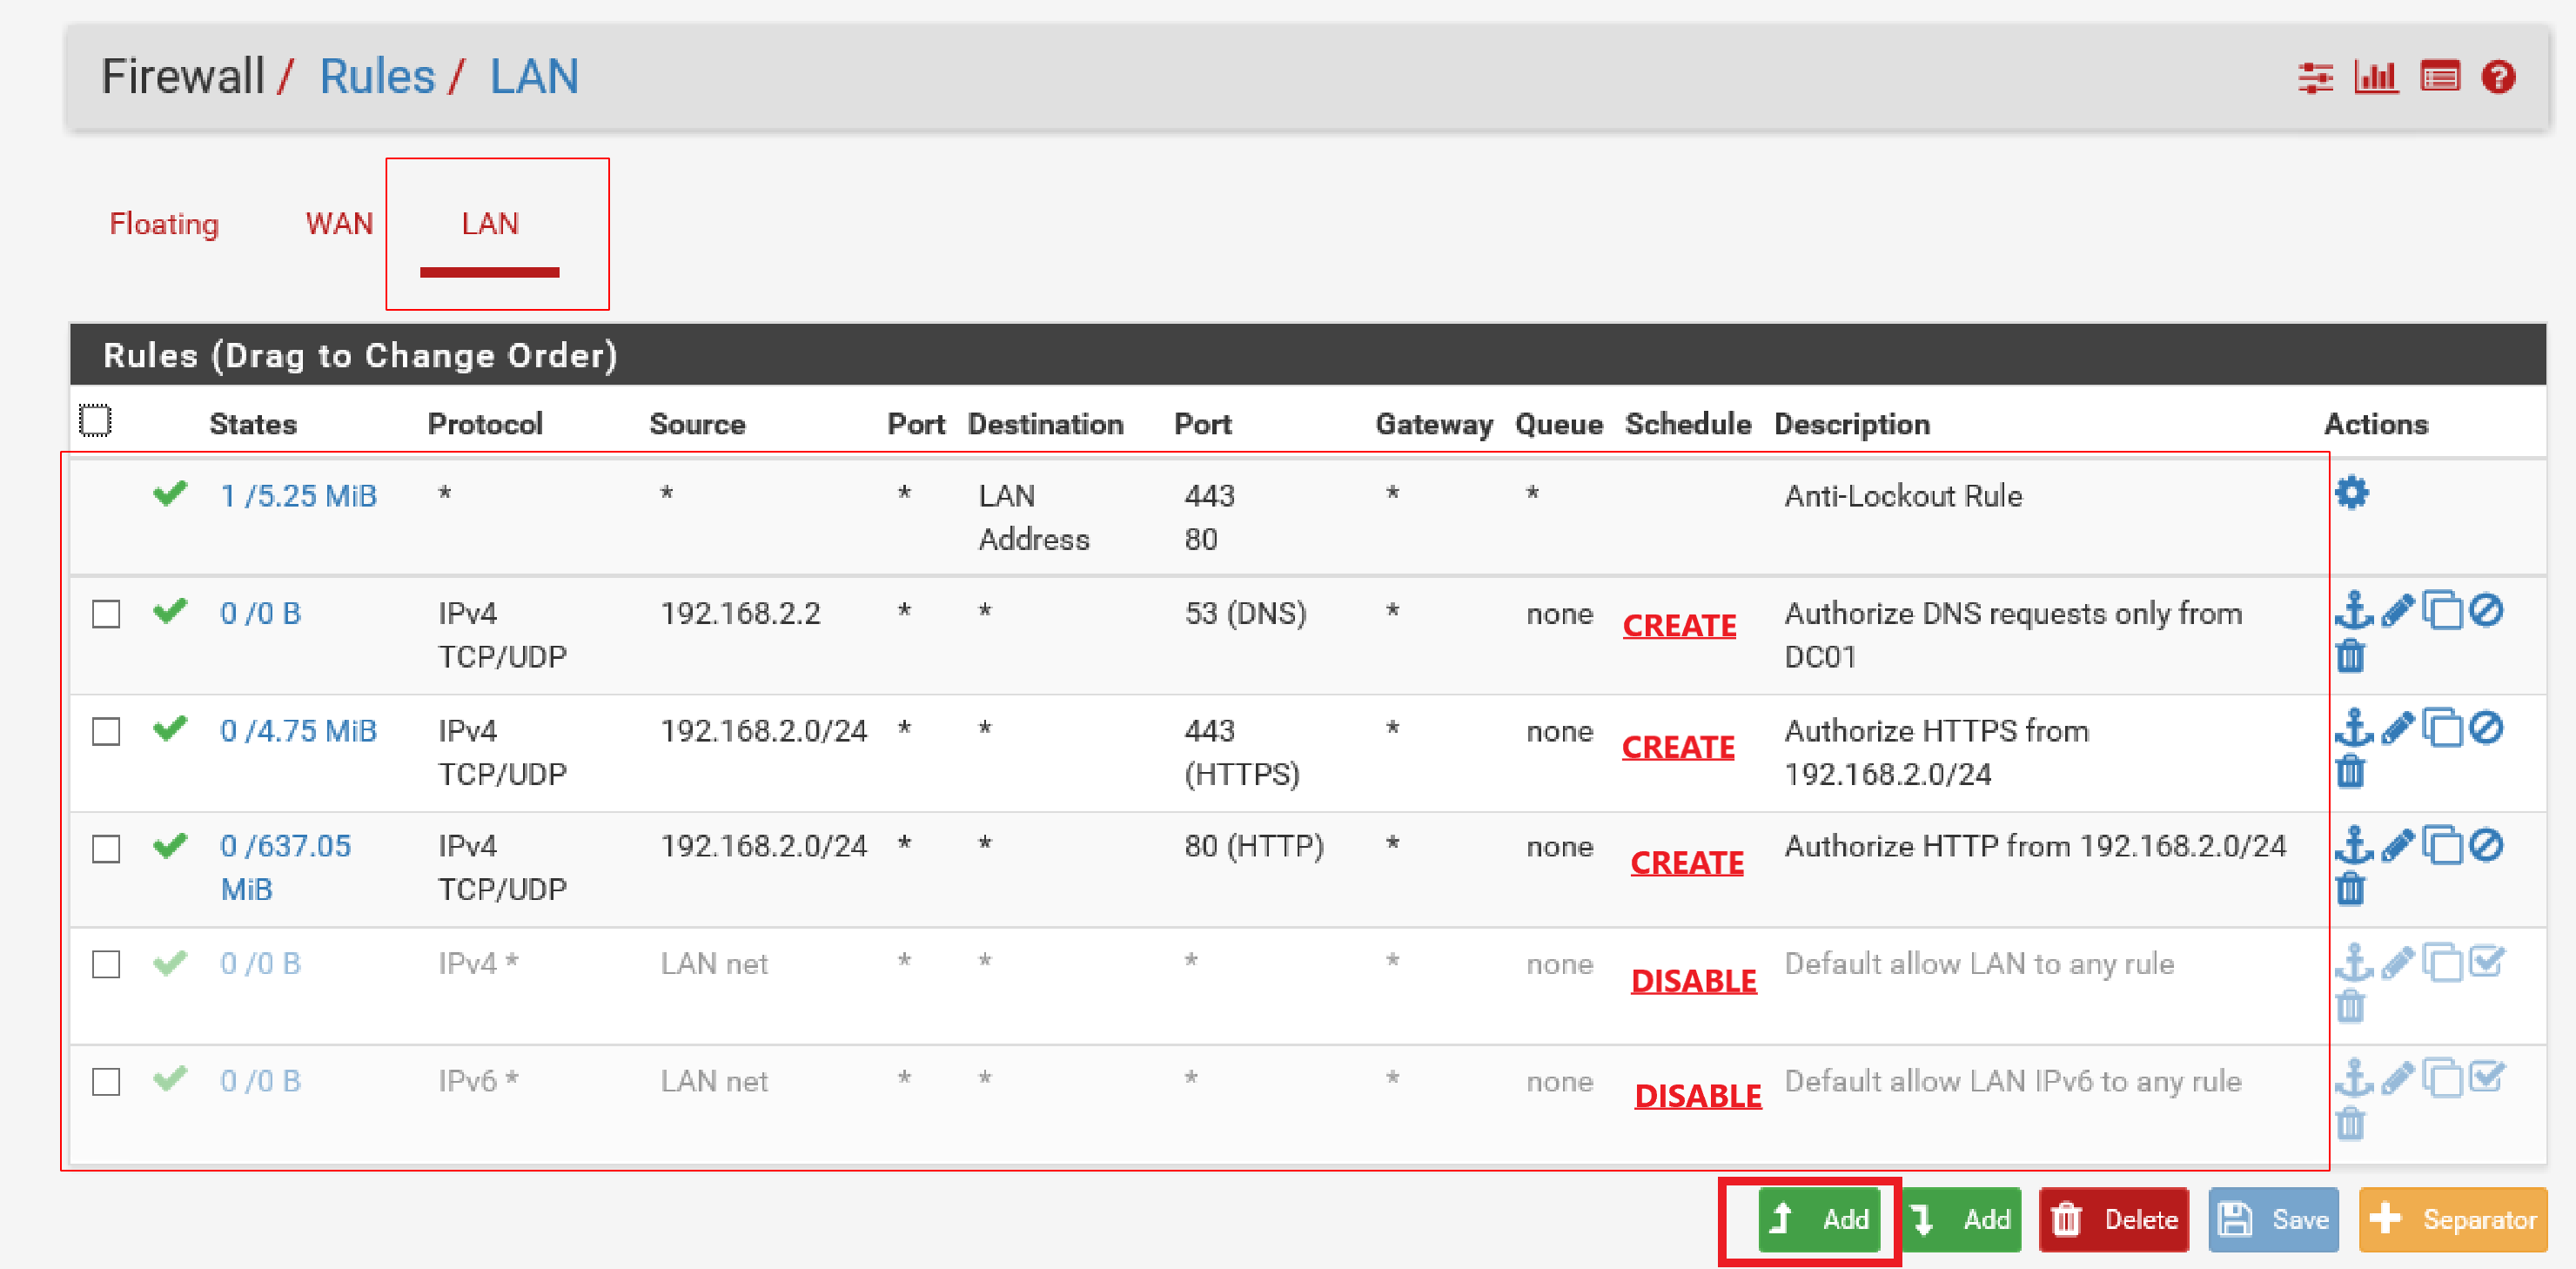
\includegraphics[scale=0.2]{Pfsense_Screeshots/22.png}
		\caption{Modification des règles de Pfsense via Windows Server}
		\label{Pfsense_Screeshots/22}
	\end{center}
\end{figure}
\FloatBarrier